\subsection*{Общая характеристика работы}

\newcommand{\actuality}{\underline{\textbf{Актуальность темы.}}}
\newcommand{\aim}{\underline{\textbf{Целью}}}
\newcommand{\tasks}{\underline{\textbf{задачи}}}
\newcommand{\defpositions}{\underline{\textbf{Основные положения, выносимые на~защиту:}}}
\newcommand{\novelty}{\underline{\textbf{Научная новизна:}}}
\newcommand{\influence}{\underline{\textbf{Практическая значимость}}}
\newcommand{\reliability}{\underline{\textbf{Достоверность}}}
\newcommand{\probation}{\underline{\textbf{Апробация работы.}}}
\newcommand{\contribution}{\underline{\textbf{Личный вклад.}}}
\newcommand{\publications}{\underline{\textbf{Публикации.}}}

\actuality\
Для~больших и~сложных программно-технических комплексов полное покрытие всех путей выполнения программы становится невозможным, поскольку эта задача соотносится с проблемой останова. Ресурсы, выделенные на~тестирование сложных программных комплексов, всегда ограничены, что приводит к~необходимости рационального  их использования. Проблема поиска подходящего компромисса  между повышением надежности разрабатываемых программных средств и~эффективным использованием ресурсов становится все актуальнее. Для~обеспечения надёжности программных средств  активно ведётся разработка новых эффективных методов и~средств автоматического тестирования, позволяющих за~реальное время предупредить и~выявить как~можно большее количество дефектов в~программе. В~настоящее время всё большее распространение получают инструменты, предназначенные для~поиска дефектов в~программном коде.

Обычно различают статический, динамический и~смешанный анализ. Под статическим анализом понимают анализ программы, не~требующий её непосредственного выполнения. Часть инструментов, таких, как~Clang Static Analyzer \cite{csa}, PVS-Studio \cite{pvs}, Cppcheck \cite{cppcheck}, Lint \cite{lint}, исследует непосредственно код программы или структуры данные, строящиеся на~его основе,~--- абстрактное синтаксическое дерево или граф потока управления. Другая часть инструментов статического анализа использует для~анализа более низкоуровневое представление программы~--- скомпилированный объектный или промежуточный код (Coverity Prevent \cite{coverity}, Svace \cite{svace}, FindBugs \cite{findbugs}). В~отличие от~статического анализа, для~динамического анализа программы требуется её выполнение~--- на~специальных входных данных, в~виртуальной машине (Valgrind \cite{valgrind}), с~использованием инструментации (AddressSanitizer \cite{asan}, ThreadSanitizer \cite{tsan}, UndefinedBehaviorSanitizer), с~использованием дополнительных библиотек или их подменой. Наконец, смешанный анализ представляет собой комбинацию статического и~динамического анализа и~используется в~таких инструментах как~Mayhem \cite{mayhem}, KLEE \cite{klee}, а~также других автоматических генераторов контрпримеров.

Перечисленные виды анализа имеют свои достоинства и~недостатки, в~частности, различные виды анализа наиболее эффективны для~поиска различных видов ошибок.

\begin{itemize}
 \item Динамический анализ наиболее хорошо зарекомендовал себя для~поиска ошибок, связанных с~многопоточностью и~управлением памятью, однако крайне затратен в~случае больших проектов. Значительным недостатком динамического анализа является необходимость явного выполнения программы, что влечёт за~собой необходимость подготовки входных данных (или их автогенерации), и~быстрый рост длительности такого анализа с~увеличением объёма проекта. Это также затрудняет интеграцию инструментов, использующих динамический анализ, в~процесс разработки, что снижает шансы быстрого обнаружения ошибки.
 \item Статический анализ позволяет эффективно производить поиск различных видов дефектов: опечаток, некорректного использования типов, проблем безопасности, неопределённого или недокументированного поведения и~многих других видов. Инструменты для~выполнения статического анализа могут быть легко интегрированы в~процесс разработки. При~этом они могут быть использованы как~индивидуальные вспомогательные инструменты разработки (например, для~подсветки кода, содержащего потенциальную ошибку), так и~в~качестве инструментов, использующихся группой разработчиков (например, для~развёртывания и~интеграции в~систему непрерывной сборки). Сравнительно небольшое время, затрачиваемое на~анализ, вкупе с~интеграцией в~рабочий процесс позволяет быстро находить дефекты в~разрабатываемых программах. Недостатком статических анализаторов является возможность выдачи ими некорректных сообщений об ошибках~--- ложных срабатываний (ошибок первого рода) и~возможность пропуска имеющихся дефектов (ошибки второго рода), вероятность которых стараются снизить при~разработке анализаторов. Вред от~ошибок второго рода очевиден, но и~ошибки первого рода играют не~меньшую роль при~оценке качества анализатора, поскольку их большое количество отвлекает разработчика на~длительное время для~просмотра ложных срабатываний, поэтому при~большом количестве ложных срабатываний инструмент может стать практически непригодным для~использования. Однако при~небольшом количестве ложных срабатываний польза от~применения анализатора в~виде снижения времени, затрачиваемого на~обнаружение ошибки, быстро перевешивает недостаток в~виде времени, затрачиваемого на~просмотр ложных срабатываний.
\end{itemize}

Первоначально распространение у разработчиков получили инструменты, использующие методы на~основе анализа синтаксического дерева программы и~её графа потока управления. Преимуществами данных методов анализа программного кода являются:

\begin{itemize}
 \item высокая скорость работы,
 \item незначительное потребление памяти,
 \item возможность его реализации в~компиляторе для~выполнения дополнительных проверок и~предупреждения программиста о~потенциально некорректном поведении компилируемого кода. Это становится возможным благодаря малому потреблению системных ресурсов, позволяющему лишь незначительно снижать производительность компилятора,
 \item возможность интеграции в~среды разработки для~осуществления анализа <<на лету>>, непосредственно в~процессе набора кода программистом, или в~качестве дополнительного инструмента для~быстрого обнаружения дефекта.
\end{itemize}

Аналогичные методы применяются в~компиляторах для~предупреждения программиста о~потенциально некорректном поведении программы, поскольку и~синтаксическое дерево, и~граф потока управления являются основными структурами данных, с~которыми работает компилятор. Однако проверка, включаемая в~состав компилятора, должна исключать возможность ложных срабатываний, т.~е. являться консервативной. Инструменты же статического анализа могут включать также и~неконсервативные проверки, с~возможностью выдачи ложных срабатываний.

Данные методы могут обнаруживать лишь очень узкие классы дефектов в~программном коде: простые ошибки, затрагивающие лишь несколько операторов, расположенных в~пределах одной функции. Это может быть простейший поиск использования неинициализированных переменных, ошибок при~преобразовании типов, потенциально лишние операции, а~также другие дефекты, для~поиска которых не~требуется анализировать циклы и~условные переходы. При~наличии циклов и~переходов в~анализируемой функции эффективность видов анализа, нечувствительных к~путям выполнения, резко падает, поскольку данные методы позволяют корректно определить достижимость одних операторов из других операторов при~выполнении программы лишь в~тривиальных случаях.

Значительно более ресурсоёмким, но и~более подробным является анализ на~основе обхода путей выполнения программы. Основы этих методов были заложены ещё в~70-х~годах. Метод символьного выполнения был предложен Джеймсом Кингом в~1976 году \cite{king76}. В~основе метода лежит идея разбиения входных данных на~классы эквивалентности в~зависимости от~встречаемых по пути выполнения условий. Метод абстрактной интерпретации, предложенный в~1977~году супругами Кузо \cite{cousot}, предполагает использовать абстрагирование данных и~их анализ на~основе алгебры решёток. Однако данные походы стали получать распространение только в~последнее время. Это связано с~увеличившейся мощностью компьютеров: время анализа растёт пропорционально количеству путей выполнения, что означает экспоненциальный рост времени анализа с~увеличением размера программы. (Вообще говоря, абсолютно полный и~точный анализ программы невозможен в~связи с~проблемой останова, независимо от~применяемого подхода.) В~отличие от~базового анализа графа потока управления, анализ путей выполнения способен учитывать условия выполнения тех или иных ветвей программы,  следствием чего являются преимущества данного вида анализа~--- его более высокая точность и~способность покрыть намного больший класс дефектов. Такие методы, как~абстрактная интерпретация и~символьное выполнение, нашли применения в~известных инструментах для~поиска дефектов, например, Coverity SAVE, Clang Static Analyzer и~многих других.

Одними из наиболее актуальных целевых языков для~статического анализа традиционно являются языки C и~C++. Причин для~этого несколько. Во-первых, это связано с~большим количеством видов потенциальных ошибок, которые может допустить программист, ведущий разработку с~использованием этих языков. Наиболее специфичными среди таких ошибок являются ошибки, связанные с~неправильной работой с~указателями~--- переполнение буфера, обращение к~неинициализированной памяти или к~памяти по некорректному адресу. Во-вторых, стандарты языков трактуют достаточно большое количество ситуаций как~не~имеющих определённого поведения (например, порядок вычисления аргументов функций может быть произвольным), что, с~одной стороны, позволяет компилятору проводить более глубокие оптимизации и~получить наибольшую скорость выполнения результирующего кода, но, с~другой стороны, требует от~программиста повышенного внимания в~процессе написания кода программы для~учёта этих особенностей. В-третьих, эти языки являются одними из самых распространённых и~известных, с~их использованием было разработано и~продолжает создаваться большое количество как~системного, так и~прикладного программного обеспечения. Кроме того, язык C является практически единственным выбором при~разработке низкоуровневых компонентов, например, компонентов операционных систем и~драйверов, что также предъявляет повышенные требования к~качеству программного кода.

\aim\ данной работы является теоретическое обоснование и исследование подходов для модификации существующего метода межпроцедурного анализа, который будет использован для построения универсального анализатора кодов программ, разработанных с использованием языков C и C++, для дальнейшего встраивания в среду автоматического тестирования, с целью повышения эффективности анализа больших прикладных программных комплексов.

Для достижения указанной цели в диссертационной работе решаются следующие {\tasks}:
\begin{enumerate}
  \item Разработка модификации метода межпроцедурного анализа программ, пригодной для реализации в многоцелевом статическом анализаторе программного кода на языках C и C++ и позволяющей использовать различные виды проверок кода с целью поиска дефектов в нём.
  \item Разработка метода межмодульного анализа программ, реализованных с использованием языков C и C++, для повышения полноты анализа многокомпонентных систем.
  \item Реализация программного обеспечения (многоцелевой анализатор и его утилиты) на основе предложенных методов с целью его промышленного и коммерческого применения для поиска дефектов в исходном коде программных комплексов.
\end{enumerate}

% \defpositions
% \begin{enumerate}
%   \item Разработка модификации метода межпроцедурного анализа программ, пригодной для реализации в многоцелевом статическом анализаторе программного кода на языках C и C++ и позволяющей использовать различные виды проверок кода с целью поиска дефектов.
%   \item Разработка метода межмодульного анализа программ, реализованных с использованием языков C и C++, для повышения полноты анализа многокомпонентных систем.
%   \item Реализация программного обеспечения (многоцелевой анализатор и его утилиты) на основе предложенных методов с целью его промышленного и коммерческого применения для поиска дефектов в исходном коде программных комплексов.
% \end{enumerate}
% 
\novelty

Научная новизна диссертации определяется получением следующих результатов, которые выносятся на защиту:
Научная новизна диссертации определяется получением следующих результатов, которые выносятся на защиту:
\begin{enumerate}
  \item Формализованы функциональные требования к разрабатываемому в данной работе методу межпроцедурного анализа.
  \item Разработана модификация метода межпроцедурного анализа программ на основе резюме для метода символьного выполнения для программ, реализованных с использованием языков C и C++. Важными особенностями разработанного метода является поддержка проверок произвольного вида и их одновременного выполнения, а также поддержка модели памяти, используемой в языках C и C++, в том числе, с учётом арифметики указателей, наследования и выравнивания полей структур.
  \item Разработан алгоритм переименования областей памяти для трансляции имён переменных между различными функциями, использующий цепочки доступа. Данный алгоритм используется для установления соответствия между регионами памяти различных объектов, используемых в функциях.
  \item Формализованы критерии достижимости и отсечения недостижимых ветвей выполнения программы с целью увеличения производительности анализатора при обработке больших графов выполнения (порядка $10^{11}$--$10^{12}$ узлов) в автоматическом режиме, а также устранения ложных срабатываний. Разработан алгоритм построения фрагментов графа выполнения, моделирующих вызов функции, с учётом ограничений на входные данные, известных на момент вызова функции. 
  \item Разработан метод межмодульного анализа программ, реализованных с использованием языков C и C++, для статического анализатора, использующего в качестве входных данных непосредственно исходный код программы. Использование промежуточного представления в виде синтаксического дерева программы позволяет производить анализ без потери информации о программе.
  \item Разработан алгоритм построения отчёта о дефекте при использовании предложенной модификации метода резюме для метода символьного выполнения. Данный метод позволяет строить информативный межпроцедурный отчёт, включающий показ переходов, выполнимых условий и представляющих интерес событий в процессе выполнения программы.
  \item Проведён сравнительный анализ метода МПА, использующего встраивание кода функции, и метода МПА, использующего её резюме. Результаты автоматического и ручного тестирования, проведённого для данных методов, показали значительное преимущество предложенного метода. Результаты также свидетельствуют об увеличении скорости поиска дефектов: то же самое количество уникальных дефектов можно находить за время, в 2--3 раза меньшее, в сравнении с методом встраивания. Ручная проверка части дефектов показала, что качество анализа при использовании метода резюме не уменьшается в сравнении с методом встраивания и составляет 80--84\%.


\end{enumerate}

\influence\ Разработаны методы анализа программ, применимые для проектов масштаба операционных систем и их наборов пользовательских приложений, реализованные в практически используемом анализаторе программного кода. Предложенные в диссертационной работе методы и алгоритмы позволяют проводить анализ программных систем объёмом порядка 5--20~млн. строк кода (или около $10^{11}$--$10^{12}$ узлов графа выполнения) в автоматизированном режиме. Данные методы и алгоритмы использованы для создания универсального анализатора кодов программ на языках C и C++. Разработан ряд проверяющих модулей с поддержкой предложенного метода межпроцедурного анализа, имеющих высокую и достаточную для практического применения точность анализа.

\underline{\textbf{Теоретическая значимость}} работы состоит в теоретическом обосновании преимущества метода резюме над методом встраивания в отношении полноты и производительности анализа. Формализованы и с помощью построенной математической модели временных затрат на межпроцедурный анализ показаны условия, при которых анализ с использованием метода резюме имеет преимущество перед методом встраивания. В работе показано, что при переходе от МПА с помощью метода встраивания к МПА с помощью метода резюме полнота анализа сохраняется. Показана возможность осуществления межмодульного анализа программ на языках C и C++ без применения компиляции их в промежуточный код.

\reliability\ полученных результатов обеспечивается экспериментальным подтверждением и последующей ручной проверкой отчётов анализатора при анализе исходного кода ОС Android версии 4.2.1. Ряд обнаруженных дефектов может быть найден с использованием других статических анализаторов, например, Coverity SAVE или Clang Static Analyzer (с режимом встраивания). Для тестирования был использован открытый исходный код, а разработанная экспериментальная система помещена в открытый доступ вместе с исходным кодом (https://github.com/helinteg/srr-clang), что позволяет воспроизвести эксперименты независимо.

\underline{\textbf{Реализация и внедрение результатов работы.}} Результаты диссертационного исследования использованы при разработке программных средств поиска дефектов в составе комплекса статического анализа, используемой подразделениями Samsung Electronics, и используется для анализа исходного кода ПО различного назначения, в частности, мобильных приложений и операционных систем, телевизионного ПО, ПО медицинских систем, и может использоваться для других программных систем, включая настольные приложения и системы управления, с целью поиска потенциальных дефектов, что подтверждается актами о внедрении.

\probation\
Основные результаты работы докладывались~на:
\begin{enumerate}
 \item 10-й Международной Ершовской конференции <<Перспективы систем информатики>> (PSI 2015) (Казань, Россия, 2015)
 \item XII Международной научно-практической конференции <<Инновации на основе информационных и коммуникационных технологий>> (INFO-2015) (Сочи, Россия, 2015)
 \item Открытой конференции по компиляторным технологиям (Москва, Россия, 2015).
\end{enumerate}


\contribution\ Все выносимые на защиту результаты получены лично автором.

\publications\ Основные результаты по теме диссертации изложены в 4 печатных изданиях~\cite{summary-impl-mine,summary-intro-mine,summary-inter-unit-mine,info-2015},
3 из которых изданы в журналах, рекомендованных ВАК~\cite{summary-impl-mine,summary-intro-mine,summary-inter-unit-mine}, 
1~--- в тезисах докладов~\cite{info-2015}. В работах \cite{summary-impl-mine,summary-intro-mine,summary-inter-unit-mine} автору принадлежат теоретические модели, обзорные разделы, описание элементов разработанных методов, а также результаты экспериментального тестирования разработанного в рамках работы ПО.
 % Характеристика работы по структуре во введении и в автореферате не отличается (ГОСТ Р 7.0.11, пункты 5.3.1 и 9.2.1), потому её загружаем из одного и того же внешнего файла, предварительно задав форму выделения некоторым параметрам

%Диссертационная работа была выполнена при поддержке грантов ...

%\underline{\textbf{Объем и структура работы.}} Диссертация состоит из~введения, четырех глав, заключения и~приложения. Полный объем диссертации \textbf{ХХХ}~страниц текста с~\textbf{ХХ}~рисунками и~5~таблицами. Список литературы содержит \textbf{ХХX}~наименование.

%\newpage
\subsection*{Содержание работы}
Во \underline{\textbf{введении}} обосновывается актуальность исследований, проводимых в рамках данной диссертационной работы, приводится обзор научной литературы по изучаемой проблеме, формулируется цель, ставятся задачи работы, сформулированы научная новизна и практическая значимость представляемой работы.

В \underline{\textbf{первой главе}} рассмотрен вопрос статического анализа компьютерных программ и, в особенности, метод символьного выполнения как один из наиболее актуальных и используемых на практике. Рассмотрены основные проблемы, возникающие при использовании данного метода, и методы их решения. Представлены и проанализированы работы, посвящённые улучшениям метода символьного выполнения, в т.~ч. наиболее близкие к тематике работы.

 картинку можно добавить так:
\begin{figure}[ht] 
  \center
  \includegraphics [scale=0.27] {latex}
  \caption{Подпись к картинке.} 
  \label{img:latex}
\end{figure}

Формулы в строку без номера добавляются так:
\[ 
  \lambda_{T_s} = K_x\frac{d{x}}{d{T_s}}, \qquad
  \lambda_{q_s} = K_x\frac{d{x}}{d{q_s}},
\]

Во \underline{\textbf{второй главе}} рассмотрен и подробно описан метод межпроцедурного анализа программ с использованием резюме для метода символьного выполнения. Разработанный алгоритм метода межпроцедурного анализа с помощью резюме для метода символьного выполнения выглядит следующим образом:

\begin{enumerate}
 \item Провести анализ вызываемой функции, получив в результате её граф выполнения.
 \item Для каждого конечного узла графа выполнения функции осуществить сбор эффектов, оказываемых на выполнение программы при выполнении данной ветви выполнения. Полученным результатом является набор ветвей резюме.
 \item В каждой точке вызова проанализированной функции создать новые узлы графа выполнения (узлы применения резюме) со следующими характеристиками:
 \begin{itemize}
  \item Дуги графа выполнения ведут из узла, соответствующего вызову функции (узел вызова) в каждый из узлов применения резюме.
  \item Каждая точка применения резюме соответствует листу графа выполнения вызываемой функции и, соответственно, своей ветви резюме.
  \item Состояние программы в каждой точке применения резюме есть композиция состояния программы в узле вызова и функции, описываемой соответствующей ветвью резюме.
 \end{itemize}
\end{enumerate}

Каждый оператор при своём выполнении производит эффект, заключающийся в изменении состояния программы. В случае анализа речь идёт о моделировании эффектов операторов, то есть о моделировании действия, которое моделируемый оператор оказывает на модель состояния программы. Сократить время анализа при использовании резюме в сравнении со встраиванием можно получить за счёт отсутствия необходимости затрачивать время на анализ эффектов, действия которых локальны или не учитываются при дальнейшем анализе. Например, связывание символьного значения с выражением имеет только локальный эффект, поскольку все выражения становятся неактивными при выходе из контекста анализа функции. Аналогично, локальный эффект имеют записи в локально видимую память и т.~д. Кроме того, модель анализатора заведомо допускает упрощения, поскольку анализатор не может досконально смоделировать поведение программы. Это означает, что ряд эффектов операторов не будет учтён, т.~е. на моделирование некоторых эффектов операторов будет затрачено время, однако результат этого моделирования не будет отражён в изменении состояния. Учёт этих упрощений и ограничений анализатора позволяет устранить непроизводительные затраты времени, поскольку при применении резюме непроизводительные вычисления не выполняются повторно. Возможно, однако, что некоторые эффекты самого применения резюме не могут быть учтены моделью анализатора и также будут отнесены к непроизводительным вычислениям. Тем не менее, время, затрачиваемое на применение резюме, по-прежнему не будет превышать время, требуемое на анализ вызова функции методом встраивания. Это объясняется тем, что набор эффектов, получаемых в результате применения резюме, включается строго или совпадает с набором эффектов, моделируемых при анализе методом встраивания.

В данной работе рассмотрен следующий набор эффектов, оказывающих влияние на состояние анализируемой программы в процессе её выполнения:

\begin{enumerate}
 \item Принятие решений о выборе пути выполнения. Выбор пути выполнения сопровождается наложением ограничений на символьные значения, относительно которых принимается решение о выборе пути. Если эти символьные значения содержат ссылки на внешние по отношению к вызываемой функции регионы памяти, накладываемые ограничения должны быть отражены в резюме. Кроме того, как было показано выше, каждое принятие решения влияет на присутствие и порядок операторов в последовательности выполнения, а следовательно, и на набор эффектов, включаемых в резюме. Наконец, наложение ограничений на входные данные функции в зависимости от выбора пути выполнения позволяет сохранить контекстную чувствительность при анализе, поскольку определённые пути выполнения могут быть достижимы лишь при ограниченном наборе входных значений аргументов функции и значений, находящихся во внешней по отношению к ней памяти.
 
 \item Модификация регионов памяти с областью видимости, отличной от локальной, то есть находящихся в статической или глобальной области видимости, принадлежащих куче, а также модификация аргументов, переданных по неконстантному указателю или неконстантной ссылке, и областей памяти, относящихся к ним (возможно, с использованием арифметики указателей).
 
 \item Инвалидация регионов памяти, то есть пометка некоторых регионов как изменивших значение на неизвестное. Данное действие обычно выполняется при моделировании оператора, все эффекты которого учесть по каким-либо причинам невозможно~--- например, при вызове функции с недоступным определением.
 
 \item Возврат вызываемой функцией некоторого значения. Это значение связывается с выражением вызова функции как элемент окружения.
 
 \item Пометки проверяющих модулей:
 
 \begin{enumerate}
  \item пометки символов, регионов памяти и символьных значений;
  \item события, которые необходимо проверить отложенно, когда контекст вызываемой функции станет достаточно определён для того, чтобы утверждать наличие потенциального дефекта;
  \item иные действия, связанные с процедурами проверок (в зависимости от логики работы проверяющего модуля).
 \end{enumerate}
 
\end{enumerate}

Поскольку проверяющие модули самостоятельно отвечают за свои данные, логику обработки резюме для проверок имеет смысл включать непосредственно в логику работы этих модулей.

Одним из результатов сбора резюме являются пары <<регион памяти~--- символьное значение>>. В результате актуализации символьных значений из резюме могут получиться символьные значения, имеющие диапазон, отличный от диапазона этого символьного значения в контексте вызывающей функции. Это является следствием того, что при моделировании условий внутри вызываемой функции может произойти разделение входных данных функции (аргументов и внешних переменных) на классы эквивалентности.

Введём следующие обозначения:
\begin{itemize}
 \item $n$ – количество ветвей выполнения, полученных в резюме анализа вызываемой функции,
 \item $i$ – номер ветви выполнения, где $0 \leqslant i < n$,
 \item $p_i$ – количество символьных правосторонних входных значений в $i$-ой ветви выполнения,
 \item $j$ – номер символьного значения, где $0 \leqslant j < p_i$,
 \item $s_{ij}$ – символьное значение с номером $j$ в $i$-ой ветви выполнения,
 \item $r_{\text{входные}\ ij}$ – множество значений для $s_{ij}$ в контексте вызывающей функции в точке непосредственно перед вызовом функции,
 \item $r_{\text{резюме}\ ij}$ – множество значений для $s_{ij}$ в контексте вызываемой функции,
 \item $state_{\text{входное}}$~--- состояние программы в контексте вызывающей функции в точке непосредственно перед вызовом функции,
 \item $state_{\text{выходное}}$~--- состояние программы после вызова функции (после применения резюме).

\end{itemize}

Тогда при применении $i$-й ветви выполнения резюме:

\begin{equation*}
\label{result_sval}
 \forall i \in [0; n], \forall j \in [0; p_i]:\ r_{\text{выходные}\ ij} =  r_{\text{входные}\ ij} \cap r_{\text{резюме}\ ij},
\end{equation*}

то есть результирующее множество является пересечением множеств входных конкретных значений символического значения и множества конкретных значений символического значения из применяемой ветви резюме.

В случае, если результирующее множество конкретных значений является пустым хотя бы для одного символического значения, то данная ветвь выполнения является недостижимой и не принимается в дальнейшее рассмотрение, что может быть выражено формулой:

\begin{equation*}
 \label{empty_set}
 (\exists i, j: r_{\text{входные}\ ij} \cap r_{\text{резюме}\ ij} = \varnothing)  \Rightarrow (state_{\text{входное}} \nrightarrow state_{\text{выходное}})
\end{equation*}

Пусть некоторое значение относится к региону памяти. Поскольку при передаче аргумента в функцию не по значению его значение может измениться, необходимо различать входное значение региона до его изменения в функции и выходное значение. Для получения информации о разбиении данных на классы эквивалентности мы отслеживаем событие потери актуальности (активности) и определяем диапазон возможных значений символа, связанного с данным регионом, в данной ветви выполнения. При этом первое событие потери активности соответствует диапазону входных значений, а последнее соответствует диапазону выходных значений, причём если они совпадают, это означает, что никаких присваиваний или инвалидаций региона входного символа не было, и входной диапазон является также выходным диапазоном. Данный метод позволяет избежать использования сложных алгоритмических схем для сбора входных и выходных значений аргументов функций, а также входных значений глобальных регионов памяти. Сбор выходных значений также бывает необходимо проводить по окончании пути выполнения функции. Это необходимо для обработки символьных значений, привязанных к региону памяти непосредственным присваиванием или иным видом связывания. Для этого используется итерация по хранилищу с сохранением диапазонов внешних по отношению к функции регионов памяти в резюме. 

Под инвалидацией региона памяти мы понимаем связывание с данным регионом нового символа, без наложенных на него ограничений, т.~е. способного принимать произвольные значения. Поскольку символьные значения, связанные с регионами памяти, обрабатываются при завершающем проходе по хранилищу, а значения регионов, актуальные до инвалидации, обрабатываются по событию потери активности, непосредственно предшествующему событию связывания нового значения, инвалидация обрабатывается автоматически, и дополнительных действий для обработки инвалидаций регионов памяти не требуется.

Обработка события возврата функцией значения достаточно тривиальна. Результирующее символьное значение сохраняется в резюме целиком, а ограничения, накладываемые на него и на его части, обрабатываются отдельно.

За хранение данных проверок проверяющие модули отвечают самостоятельно. Основными видами данных проверок является отметка отложенной проверки и данные состояния проверки. Отложенные проверки используются для выдачи предупреждений в тех ситуациях, когда из-за отсутствия данных о контексте вызова невозможно однозначно утверждать наличие дефекта или его отсутствие. Данные состояния используются для построения нового состояния проверки при применении резюме. 

В результате сбора резюме на предыдущем шаге мы получаем некоторое множество регионов памяти, с которыми связаны некоторые символьные значения. Кроме того, регионы памяти сами могут входить в символьные значения как их составная часть. Однако, полученные регионы памяти адресуются в контексте объявлений имён внутри функции. В контексте вызывающей функции эти регионы могут иметь уже другое значение, то есть регионы, используемые внутри функции, являются относительными по отношению к вызывающей функции. Так, например, в контексте вызываемого метода класса регион памяти, связанный с указателем \texttt{this}, будет адресоваться безотносительно какого-либо объекта, а в контексте вызывающей функции этот регион будет регионом, в котором находится объект, метод которого вызывается. Аналогично, аргумент функции, фигурирующий в ней как самостоятельная переменная, (и, соответственно, как самостоятельный регион памяти), может быть подрегионом в контексте вызывающей функции~--- полем структуры, элементом массива. Кроме того, с регионом памяти в контексте вызываемой функции может быть связан не символ, относящийся к региону памяти, а константа, символьное выражение или иное значение, не имеющее в своей основе регион аргумента. Всё это означает, что для корректного применения резюме необходимо производить актуализацию символьных значений, то есть их перевод из контекста имён и значений вызываемой функции в контекст имён и значений вызывающей функции.

Идея актуализации заключается в следующем. Пусть имеется символьное значение. В его состав могут входить символы, регионы памяти и константы. Они, согласно модели анализатора, образуют дерево. Непосредственно актуализации подвергаются только регионы памяти. Таким образом, в символьном значении происходит подмена регионов памяти, содержащихся в нём, на актуализированные. Затем, если это возможности, символы полученного символьного выражения вычисляются в константы, заменяя исходные поддеревья. Данную процедуру можно выразить следующим алгоритмом:

\begin{enumerate}
 \item Для всех регионов памяти, содержащихся в символьном значении:
 \begin{enumerate}
  \item Создать новый регион, являющийся актуализацией данного региона
  \item Заменить в символьном значении исходный регион актуализированным
 \end{enumerate}
 \item Для всех символов, содержащихся в символьном значении, полученном на шаге 1:
  \begin{enumerate}
  \item Проверить, не вычисляется ли символ в константу
  \item Если символ вычисляется в константу, заменить данный символ вычисленной константой.
 \end{enumerate}

\end{enumerate}

Схемы применения резюме, описанные выше, затрагивают отсечение недостижимых ветвей выполнения программы и уточнение множества конкретных значений для символьных значений. Однако для того, чтобы анализатор имел возможность выполнять проверки при вложенном вызове функции, необходима доработка проверяющих модулей. Для получения проверяющими модулями возможностей анализа при использовании резюме мы вводим две дополнительных функции обратного вызова. Первая из них (названная \texttt{evalSummaryPopulate}) вызывается для сбора резюме проверяющим модулем, вторая (названная \texttt{evalSummaryApply}) вызывается при применении резюме.

Проверяющий модуль, имеющий возможность выполнения действий при событии \texttt{SummaryPopulate}, должен сохранить информацию, которая может понадобиться для обновления состояния или для выполнения отложенной проверки. Информация, содержащая в резюме, не освобождается до окончания работы анализатора, поэтому проверяющий модуль может использовать произвольный формат хранения данных, лучшим образом отвечающий задаче проверки. Как показала практика модификации проверяющих модулей, для каждой проверки, проводимой модулем, в GDM обычно помещается две дополнительных записи, которые затем будут использоваться для заполнения резюме~--- для обновления состояния и для отложенной проверки. В качестве примера рассмотрим проверку двойного закрытия файлового дескриптора. В резюме помещаются две секции: первая отвечает за обновление состояния дескриптора (является ли он открытым или закрытым), а вторая~--- за выполнение отложенной проверки: в ней запоминаются события закрытия дескрипторов, исходное состояние которых неизвестно.

При обработке события \texttt{SummaryApply} проверяющий модуль должен произвести обновление состояния в соответствии с информацией, хранящейся в выбранной ветви резюме. Так, если при выполнении вызова функции дескриптор был закрыт, он должен быть помечен как закрытый в состоянии вызывающей функции. Если же в контексте вызывающей функции уже известно, что дескриптор закрыт, то отложенная проверка должна выдать предупреждение.

Интерес представляет сравнение двух методов обработки данных проверяющими модулями. Определим два вида проверок формально.

Проверку при использовании метода встраивания определим следующим образом. Пусть имеется граф выполнения программы в виде дерева. Алгоритм поиска осуществляет обход дерева от корня к листу по пути $w$ без возврата, собирая ограничения, наложенные на входные данные, и отслеживая изменение состояния программы в каждом узле графа выполнения. Алгоритм поиска выдаёт срабатывание в случае обнаружения нарушения заданного для него условия корректности состояния программы в заданной точке, таким образом представляя дефект конъюнкцией $pre_w \wedge node_w$, т.~е. отображением множества значений входных данных функции на узел графа выполнения, состояние которого нарушает условие корректности программы.

Проверку при использовании метода резюме определим как проверку при использовании метода встраивания для функции верхнего уровня и отложенную проверку при использовании межпроцедурного вызова. Под отложенной проверкой понимается дополнительная проверка всех узлов графа выполнения вызываемой функции в узле применения резюме с актуализацией состояния в данных узлах с учётом контекста вызова и актуализированных ограничений на момент выхода из вызываемой функции. Отложенная проверка и обычная проверка производятся с использованием одного критерия корректности состояния программы.

\textbf{Теорема 1}. Если при использовании проверки с помощью метода встраивания результатом проверки является предупреждение, выданное в некотором узле графа выполнения программы, то при использовании метода резюме для той же функции верхнего уровня и того же набора вызываемых функций результатом проверки методом резюме также является предупреждение, выданное в узле графа выполнения вызывающей функции или в одном из узлов графов выполнения вызываемых функций.

\textbf{Теорема 2}. При использовании отложенной проверки в конце анализа функции верхнего уровня при использовании МПА методом встраивания и МПА методом резюме множества срабатываний совпадают.

Важным элементом работы статического анализатора является построение отчёта. При анализе программы методом анализа её путей выполнения необходимо выполнять построение подробного отчёта, однозначно указывающего условия, при которых проявляется дефект, и соответствующий им путь выполнения. При использовании межпроцедурного анализа методом встраивания путь, проходимый внутри функции, отображается в графе выполнения как часть общего пути выполнения, поэтому проблем при построении пути при генерации отчёта не возникает. Однако при применении метода резюме возникает проблема потери информации о части пути, проходимом внутри вызываемой функции, поскольку явного построения поддеревьев графа выполнения программы более не происходит. Для построения отчёта  при межпроцедурном анализе методом резюме в настоящей работе предложен следующий метод.

Задачей проверяющих модулей является отложенная проверка: на основе резюме вызываемой функции и состояния на момент вызова проверяющий модуль должен сделать вывод о необходимости выдачи предупреждения (срабатывании). Имеется два варианта срабатывания проверки. В первом случае выдача предупреждения происходит внутри вызываемой функции. Допустим, что уровень вложенности вызова равен единице. Такое допущение допустимо, поскольку к нему можно свести стек вызовов произвольного уровня вложенности. В этом случае конечной точкой трассы является узел графа выполнения вызываемой функции. В случае, если этот узел известен, от него можно построить трассу до корневого узла графа выполнения. Данная трасса-подграф будет являться путём, проходимым внутри функции при выполнении программы до критической точки. Второй случай предполагает построение пути при необходимости показать путь внутри вызванной функции целиком, от точки входа до точки выхода. Данная задача сводится к первой при условии, что в качестве конечной точки выбирается лист графа выполнения, соответствующий выбранной ветви выполнения резюме. 
Таким образом, для корректного построения пути при моделировании вложенного вызова функции достаточно иметь информацию или об узле графа выполнения вызываемой функции, для которого выдаётся срабатывание, или о листе графа выполнения, который относится выбранный путь выполнения при применении резюме. Для этого достаточно хранить ссылку на этот узел. В случае построения пути изнутри вызываемой функции за хранение ссылки может отвечать проверяющий модуль, генерирующий срабатывание. В случае построения полного пути по вложенному вызову ссылку на лист графа выполнения вызываемой функции можно хранить в узле применения резюме в качестве дополнительной информации.


В \underline{\textbf{третьей главе}} приводится описание разработанного метода межпроцедурного анализа программ с использованием непосредственно исходного кода, а также рассматриваются проблемы, возникающие при межпроцедурном анализе крупных программных комплексов, и методы их решения. Межпроцедурный анализ можно разделить на две категории в зависимости от области поиска определений вызываемых функций: на внутримодульный и межмодульный. Внутримодульный анализ подразумевает поиск доступных определений функций только в анализируемом модуле трансляции, тогда как в случае межмодульного анализа поиск определений может производиться и в других модулях трансляции. Очевидно, что в случае внутримодульного анализа анализатору может быть доступна лишь часть пользовательских определений функций, несмотря на потенциальную доступность исходного  кода моделируемых функций. При межмодульном анализе потенциально недоступными являются лишь библиотечные функции с недоступным исходным кодом. Межмодульный анализ позволяет находить различные классы дефектов программного кода, не обнаруживаемые при внутримодульном анализе или труднообнаружимые с его помощью, в т.~ч. ошибки интеграции модулей и подсистем программы или программного комплекса, некорректное использование программных интерфейсов (API). Межмодульный анализ становится особенно полезным для языков программирования, допускающих раздельную компиляцию исходных файлов, поскольку в этом случае информация о программе, содержащаяся в одном исходном файле, становится крайне ограниченной и затрагивает лишь малую часть программного проекта, в число которых входят C и C++.

В результате проведённого исследования была разработана архитектура анализатора, позволяющего производить межмодульный анализ программы на языках C и C++ и использующем для анализа непосредственно исходный код программы. Разработанная схема межмодульного анализа интересна тем, что позволяет использовать различные алгоритмы межпроцедурного анализа, т.~е. как анализ методом встраивания, так и анализ методом резюме, без каких-либо дополнительных модификаций как самого алгоритма межпроцедурного анализа, так и проверяющих модулей.

Единицей анализа в анализаторах исходных кодов обычно является транслируемый модуль, представляющий собой препроцессированный файл исходного кода. Однако для выполнения межмодульного анализа информации, содержащейся в одном транслируемом модуле, недостаточно. Необходимо знать расположение определений функций, необходимых для анализа других функций. Кроме того, необходимо знать не только имя и путь к файлу, где располагается определение функции. Для корректного построения импортируемого синтаксического дерева файла с исходным текстом необходимо знать, например, аргументы команды сборки файла, расположение включаемых файлов, использовавшихся для построения, и некоторую другую информацию.

В данной работе реализован трёхфазный анализ с сохранением промежуточных результатов в файлах в директории проекта. Анализ разделяется на фазу сборки, фазу предобработки данных и непосредственно сам анализ исходных кодов. На рисунке \ref{xtu-idef0} представлена схема взаимодействия инструментов, используемых на различных фазах анализа, в виде диаграммы IDEF0. На этой схеме модули, реализованные в данной работе полностью, обозначены белым цветом, а серым обозначены модули, существовавшие ранее и доработанные для использования при межмодульном анализе: \texttt{clang} является непосредственно статическим анализатором, использованным для реализации межмодульного анализа, а Perl-скрипт \texttt{ccc-analyzer} входит в состав вспомогательного пакета \texttt{scan-build} и служит для формирования командной строки запуска статического анализатора \texttt{clang} и его запуска.

\begin{figure}[h]
 \label{}
 \centering
 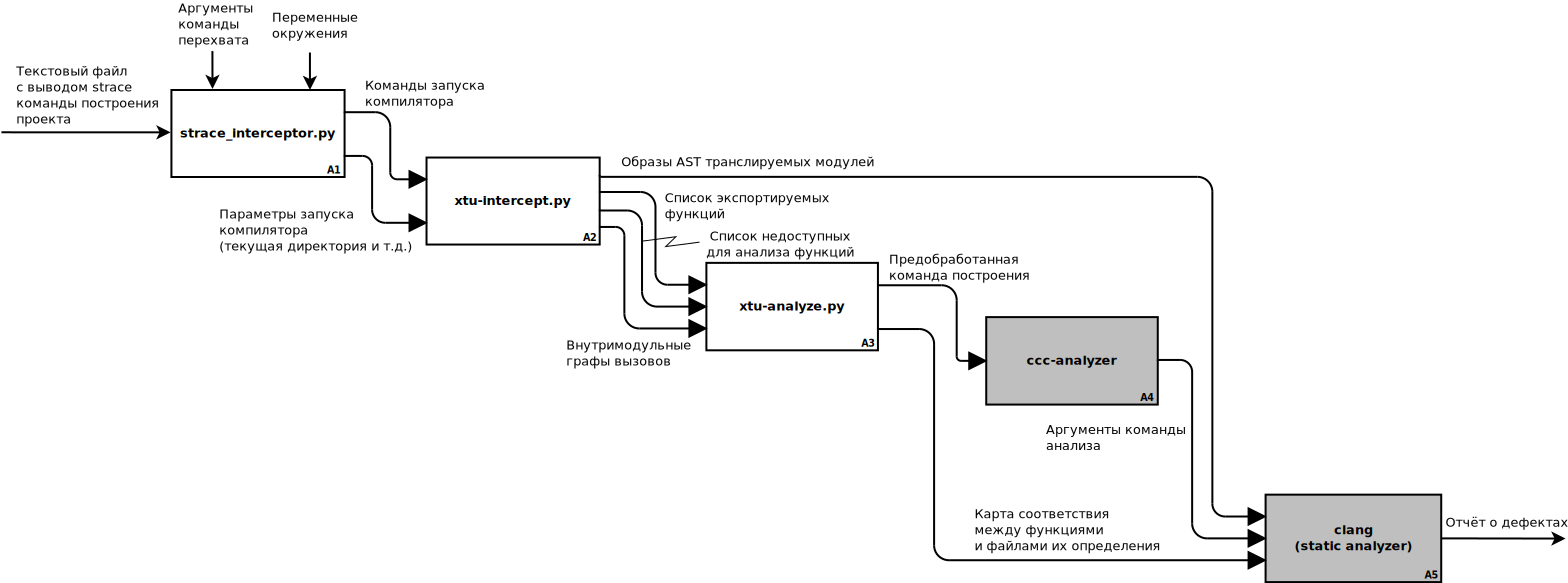
\includegraphics[width=\linewidth]{../Dissertation/images/xtu-idef0}
 \caption{IDEF0-диаграмма взаимодействия разработанных программных инструментов при межмодульном анализе}\label{xtu-idef0}
\end{figure}

На фазе сборки специальными инструментами собирается информацию о транслируемых модулях, которые должны быть проанализированы. Для этого сначала инструментом, использующим утилиту \texttt{strace}, производится перехват вызовов компилятора во время построения проекта. Затем для каждой обнаруженной команды сборки другой инструмент, использующий (API) Clang, записывает сигнатуры видимых извне (экспортируемых) определений функций данного модуля трансляции и сигнатуры используемых (импортируемых) функций, определения которых в данном модуле трансляции недоступны, в служебные файлы в директории проекта. Этот же инструмент для каждой обнаруженной функции строит локальный граф вызовов, который также сохраняется в служебный файл. На фазе сборки дополнительно создаются образы абстрактных синтаксических деревьев для всех модулей трансляции, что упрощает дальнейший импорт и позволяет избежать повторных вызовов компилятора для каждого импортируемого файла.

Необходимо учитывать целевую архитектуру сборки для каждого файла исходных кодов. Сборка одного и того же файла может выполняться одновременно для нескольких архитектур в пределах одной сессии сборки. Это значит, что для корректного импорта определения функции необходимо различать целевые тройки (target triple) цели сборки файла.  использовать определения функций из файлов, предназначенных для разных архитектур нельзя, поскольку определения встроенных и пользовательских типов для них могут не совпадать. Кроме того, один и тот же модуль трансляции может собираться несколько раз в рамках сборки для одной архитектуры. При этом также могут быть использованы различные директивы препроцессора и включаемые файлы, что может привести к потенциальной несовместимости импортируемого и импортирующего синтаксических деревьев. Все эти факторы означают, что выбирать модуль трансляции для импорта определения функции надо крайне осторожно. Для решения этой проблемы можно предложить несколько способов. В настоящей работе было использовано менее общее, но более простое в реализации решение, для которого достаточно знать, объектные модули каких архитектур могут компоноваться друг с другом. После построения такой матрицы, можно различать определения функций по тройке <путь к файлу, сигнатура функции, целевая архитектура>, и использовать эту тройку для выбора нужного определения функции и его импорта. Этот подход, не решает проблемы, связанной с использованием различных опций компилятора для одной и той же архитектуры, поскольку выбираться будет только один файл. Другим, и более общим решением видится поддержка <<дерева сборки>>. В этом случае на фазе сборки отслеживается полное дерево компиляции, ассемблирования и компоновки (и, возможно, сборки в бинарный образ) для объектных файлов верхнего уровня.

Фаза предобработки данных необходима для обработки служебной информации, собранной на фазе сборки. На этой фазе строится соответствие между сигнатурами импортируемых функций. Как только соответствие становится известным, мы можем построить глобальный граф вызовов с использованием локальных графов вызовов, которые были сгенерированы на предыдущей фазе. Каждый узел графа вызовов, таким образом, представляет собой тройку <файл определения, сигнатура функции, архитектура>. После этого выполняется топологическая сортировка построенного глобального графа вызовов. Сначала анализируются функции верхнего уровня, затем функции, участвующие в рекурсивных цепочках вызовов, а затем~--- функции нижнего уровня. При этом сортируются не сами функции, а файлы, их содержащие, поскольку анализ отдельных функций из файла означает многократную загрузку одних и тех же файлов. И, наконец, после фазы предобработки данных запускается анализ модулей трансляции в топологическом порядке глобального графа вызовов.

На вход \textit{фазы анализа} поступает файл с упорядоченным набором файлов для анализа. Все эти файлы добавляются в очередь анализа в порядке следования в исходном файле, после чего полученная очередь начинает обрабатываться пулом рабочих процессов анализатора. Данная схема позволяет осуществлять анализ с очень высокой степенью параллелизма, т.~к. различные процессы не используют разделяемых ресурсов, и её производительность линейно растёт с увеличением количества процессоров (проверена масштабируемость до 32-х процессоров включительно). Каждый анализатор из пула анализирует свой транслируемый модуль, подгружая определения функций и структур данных, от которых они зависят, по мере необходимости.

В данной разработке был реализован межмодульный анализ с использованием реализации класса \texttt{ASTImporter}, который отвечает за слияние синтаксических деревьев различных транслируемых модулей и уже был частично реализован в Clang. Реализованная функциональность была расширена, т.~к. значительная часть необходимых функций не была реализована ранее. В результате появилась возможность полноценного импорта фрагментов синтаксических деревьев функций в основной контекст синтаксического дерева. Когда анализатор обнаруживает функцию с недоступным определением, производится поиск сигнатуры этой функции в сгенерированном отображении. Если в результате поиска сигнатура функции была найдена, загружается синтаксическое дерево файла, содержащего определение этой функции. Затем эта функция импортируется в основной контекст синтаксического дерева вместе с необходимыми определениями и объявлениями.

Задача импорта фрагментов синтаксического дерева обычно решается с помощью поиска определения в целевом AST. Если аналогичное определение (или объявление) не найдено, оно создаётся в целевом AST с использованием специального интерфейса. Новый фрагмент является рекурсивной копией исходного, но в процессе импорта зависимостей также производится поиск в целевом контексте, и не все части нового фрагмента синтаксического дерева обязательно являются созданными заново, если они уже присутствуют в целевом AST.

Поскольку \texttt{ASTImporter} уже был частично реализован на момент разработки межмодульного анализа, этот раздел посвящён различным проблемам при импорте и их возможным методам решения. Первой проводимой операцией при импорте объявления из исходного контекста является поиск похожего объявления в целевом синтаксическом дереве. Этот поиск часто включает в себя рекурсивный обход вложенных объявлений для определения, являются ли два объявления структурно эквивалентными. В данной работе, однако, испытан ряд простых и легковесных эвристик, ускоряющих поиск за счёт частичного отказа от рекурсивного обхода. Рекурсивная проверка структурной эквивалентности выполняется только в случае, если эти эвристики не смогли однозначно показать различие или эквивалентность. Во-первых, если два объявления имеют различные разновидности, они, очевидно, не являются структурно эквивалентными. У этого правила, однако, есть одно исключение: класс С++ может быть импортирован как структура языка C и наоборот в случае, если это POD-структура и целевой и исходный контексты имеют различные языковые настройки. Но это исключение может быть проверено отдельно. Во-вторых, если два объявления имеют различные имена, их можно определённо считать различными без дальнейшего просмотра. В-третьих, в большинстве случаев объявления с совпадающими местоположениями в исходных файлах являются эквивалентными, за исключением специализируемых шаблонов. Основная проблема этой эвристики заключается в обработке конфликтующих объявлений.

Если эвристика не сработала, происходит возврат к рекурсивному обходу, что является одной из основных проблем импорта. Для импорта объявления необходимо сначала импортировать его контекст объявления. Этот контекст, в свою очередь, может иметь большое количество вложенных объявлений и их зависимостей. В результате происходит массовый рекурсивный импорт зависимостей как самого объявления, так и его контекста. Иногда встречаются циклические зависимости, образуемые опережающими объявлениями.

При импорте структуры или класса для создания его раскладки в памяти необходимо соблюдать порядок объявления полей в структуре, для чего поля структуры должны импортироваться в порядке объявления. Однако, если поле структуры имеет некоторый сложный тип, импорт этого типа может при рекурсивном импорте вызвать импорт другого поля структуры, например, при импорте метода, использующего это поле. В этом случае определение поля-зависимости импортируется  вне очереди импорта определений полей. Подобное поведение является нежелательным, поскольку нарушает раскладку структуры, что, в свою очередь, ведёт к различным ошибкам и невыполнению условия структурной эквивалентности. Для решения этой проблемы определения полей определения структуры переупорядочиваются после того, как определение структуры было полностью импортировано, в соответствии с их порядком в импортируемой структуре.

Код, успешно прошедший компиляцию и компоновку, может содержать несовместимые друг с другом определения. Проблема при наличии конфликтующих определений заключается в выборе стратегии поведения анализатора. Первой стратегией может стать выдача предупреждения об обнаружении конфликтующего определения с последующим завершением работы анализатора или пропуском импорта данного определения. Несмотря на логичность такого подхода, данная стратегия имеет недостаток: разработанный программный код, возможно, всё равно имеет смысл проанализировать, поскольку его работоспособность, как правило, проверяется при тестировании. Вторая стратегия заключается в разрешении конфликтов между определениями. Её недостаток заключается в том, что у анализатора может не быть данных о программе для корректного разрешения конфликта.


В \underline{\textbf{четвертой главе}} приведены результаты и методики тестирования программного обеспечения, реализующего разработанные методы.

Использование межмодульного анализа резко увеличивает количество требующих анализа путей программы и представляет интерес при сравнении производительности и качества межпроцедурного анализа методом встраивания и разработанного автором метода резюме. Таким образом, в данной работе рассматривается решение проблемы межмодульного анализа для случая использования анализатором непосредственно исходного кода программы.


В \underline{\textbf{заключении}} приведены основные результаты работы, которые заключаются в следующем:
\begin{enumerate}
 \item Результат номер один.
 \item Результат номер два.
 \item Результат номер три.
% и так далее, если нужно
\end{enumerate}


%\newpage
\renewcommand{\refname}{\large Публикации автора по теме диссертации}
%\nocite{*}
%\insertbiblioauthor                          % Подключаем Bib-базы
\insertbibliofull
